\documentclass[a4paper,oneside,11pt]{book}

\usepackage[brazil]{babel}
\usepackage[latin1]{inputenc}
\usepackage[T1]{fontenc}
\usepackage{graphicx}
\usepackage{amsfonts}
\usepackage{amssymb} 
\usepackage{indentfirst} 	
\usepackage{caption}
\usepackage{url}
\usepackage{multirow}
\usepackage[ruled, portugues]{algorithm2e} % para algoritmos
\usepackage{fancyhdr}
\usepackage[small,compact]{titlesec} 	   % t�tulos menores e compactos
\setlength{\textheight}{235mm}
\setlength{\textwidth}{150mm}
\voffset -10mm
\hoffset -10mm



%\usepackage{subfigure}
%\usepackage{subfig}
%\usepackage{wrapfig}
%\usepackage{theorem}
%\usepackage{graphics}
%\usepackage{amsmath}


%estilos de bibliografia
%\bibliographystyle{plain}
%\bibliographystyle{sbc}
\bibliographystyle{abnt-alf}

%\bibliographystyle{abnt-num}

% para melhorar o posicionamento das figuras no texto
\renewcommand{\topfraction}{0.85}
\renewcommand{\textfraction}{0.1}
\renewcommand{\floatpagefraction}{0.75}


\begin{document}

\sloppy

% set the space between lines to 1.24
\renewcommand{\baselinestretch}{1.24}
\normalsize 

%\setcounter{page}{0} 
%\pagenumbering{roman}

% set page style with page number
\setcounter{page}{1} 
\pagenumbering{arabic}
\pagestyle{plain}
\pagestyle{empty}

\begin{titlepage}
\begin{center}
Universidade Federal de Minas Gerais \\
Instituto de Ciências Exatas \\
Departamento de Ciências da Computação \\
\end{center}
\vspace{5em}
\begin{center}
{Raphael Ottoni Santiago Machado de Faria}\\ 
\vspace{10em}
{MONOGRAFIA DE PROJETO ORIENTADO EM COMPUTAÇÃO I} \\
\vspace{1em}
\textbf{Rastreamento por telefonia móvel utilizando Android} \\
\hspace{.45\textwidth} % posicionando a minipage
\vfill
Belo Horizonte -- MG \\
2010 / 2º semestre
\end{center}
\end{titlepage}
 
%\include{dedicatoria}\clearpage
%% Agradecimentos - é so para as pessoas que contribuiram relevantemente
% para a elaboração do trabalho
\pretextualchapter{Agradecimentos}

\begin{minipage}{\textwidth}
    Agradeço aos meus pais, pelo amor incondicional. \\
    Aos meus professores, pelos conhecimentos adquiridos. \\
     E finalmente aos colegas de curso pela convivência e trocas de experiências.
\end{minipage}

\clearpage
%\begin{abstract}
	
    This paper aims to create a scalable and robust  tracking system for the mobile phone network, using \emph{smartphones} with the \emph{Android} operational system.
The ideia is to add a functionality of execution of remote commands to the tracking system, thus creating a wider range of applications and possibilities. An sample of those new 
features would be in the theft case, because with this functionality the cellphone  owner would easily erase his private information such as contacts, messages and data. 

    \par
    \textbf{Keywords}: Android, Pattern: Command, Java, Google App Engine, Cloud Computing, Tracking, mobile network	
\end{abstract}
\clearpage

\begin{center}

{\bf Resumo}
\end{center}

Este trabalho apresenta ... escrever um bom resumo ap\'os finalizar a escrita do texto. 


\renewcommand{\figurename}{Figura}

\tableofcontents
%\clearpage % increment page number
\listoffigures
% add the list of figures to the table of contents
\addcontentsline{toc}{chapter}{\listfigurename} 
%\clearpage % increment page number
\listoftables
% add the list of tables to the table of contents
\addcontentsline{toc}{chapter}{\listtablename} 
%\cleardoublepage % add a blank page


% set headings
\pagestyle{fancy}
\lhead[\fancyplain{}{\footnotesize\thepage}]
      {\fancyplain{}{\footnotesize\rightmark}}
\rhead[\fancyplain{}{\footnotesize\leftmark}]
      {\fancyplain{}{\footnotesize\thepage}}

\cfoot{}

\chapter{Introdu��o} 
\label{cap:introducao}



O Cap�tulo~1 do relat�rio apresenta a introdu��o, que � possivelmente
a  principal parte do trabalho e a mais dif�cil de ser escrita.  A
introdu��o aborda v�rios assuntos.  Em primeiro lugar, a introdu��o
deve descrever o contexto do trabalho, isto �, apresentar aos leitores
o t�pico do trabalho.

A seguir, o texto deve apresentar a  motiva��o para a realiza��o deste
trabalho.  Em geral, h� dois aspectos b�sicos da motiva��o.  O
primeiro aspecto refere-se � import�ncia do trabalho do ponto de vista
pr�tico. Neste caso, o trabalho pode gerar, por exemplo, economia de
recursos, ou melhoria da qualidade da execu��o de uma tarefa, ou
melhoria de desempenho de um sistema.

O segundo aspecto da motiva��o � descrever porque o trabalho �
interessante.  Este aspecto refere-se mais ao ponto de vista te�rico
da �rea de pesquisa do trabalho. Por exemplo, h� interesse em
demonstrar um teorema novo, ou apresentar uma nova demonstra��o para
um teorema j� conhecido, ou propor um novo paradigma para uma �rea de
pesquisa, ou ainda, propor uma nova teoria para explicar algum
fen�meno.

A introdu��o deve apresentar tamb�m o objetivo do trabalho, de maneira
resumida ou completa. A escolha vai depender da organiza��o escolhida
para as demais se��es. 

A introdu��o pode apresentar ainda um resumo dos resultados.  Esta �
uma estrutura gen�rica da introdu��o. Outros formatos podem ser
adotados para trabalhos espec�ficos. A introdu��o � finalizada com a
descri��o do restante do texto, para que o leitor possa organizar sua
leitura e n�o se surpreender com o que vem pela frente. 

Este texto est� organizado da seguinte forma.  O
Cap�tulo~\ref{cap:trabalhos-relacionados} apresenta os trabalhos
relacionados � �rea de pesquisa. Este cap�tulo � essencial para
demonstrar a import�ncia do trabalho e o que j� foi desenvolvido antes
da realiza��o desse trabalho. O autor deve demonstrar neste trabalho
n�o apenas que pesquisou e conhece a bibliografia mas tamb�m deve
posicionar seu trabalho em rela��o ao desenvolvimento da �rea.

  
O Cap�tulo~\ref{cap:metodologia} apresenta a metodologia utilizada.  O
Cap�tulo~\ref{cap:resultados} apresenta os resultados alcan�ados.
Finalmente, o Cap�tulo~\ref{cap:conclusoes-trabalhos-futuros}
apresenta as conclus�es obtidas e as possibilidades de desenvolvimento
de trabalhos  futuros.
 % Introducao
\chapter{Trabalhos Relacionados} 
\label{cap:trabalhos-relacionados}




Este cap�tulo inclui muitas cita��es bibliogr�ficas. Os principais
itens de bibliografia citados s�o livros, artigos em confer�ncias,
artigos em {\it journals} e p�ginas Web. A bibliografia deve seguir o
padr�o ABNT~\cite{abnt}\footnote{Este n�o � o endere�o oficial da ABNT pois as Normas T�cnicas oficiais s�o pagas e n�o est�o dispon�veis na Web. Consulte a biblioteca.}.

A bibliografia � feita no padr�o {\tt bibtex}.  As refer�ncias s�o
colocadas em um arquivo separado, com termina��o {\tt .bib}, que �
inclu�do no arquivo fonte principal ({\tt .tex}).  Os elementos de
cada item bibliogr�fico que devem constar na bibliografia s�o
apresentados a seguir.

Para livros, o formato da bibliografia no arquivo fonte � o seguinte:

\begin{verbatim}
    @Book{linked,
      author =       {A. L. Barabasi},
      title =        "{Linked: The New Science of Networks}",
      publisher =    {Perseus Publishing},
      year =         {2002},
    }
\end{verbatim}

A cita��o deste livro se faz da seguinte forma \verb#\cite{linked}# e o resultado fica assim~\cite{linked}.
Para os artigos em {\it journals}, veja por exemplo~\cite{acmsurveys},
descrito da seguinte forma no arquivo {\tt .bib}:


\begin{verbatim}
   @article{acmsurveys,
     author = {Deepayan Chakrabarti and Christos Faloutsos},
     title = {Graph mining: Laws, generators, and algorithms},
     journal = {ACM Computing Surveys},
     volume = {38},
     number = {1},
     year = {2006},
     pages = {2-59},
     publisher = {ACM},
     address = {New York, NY, USA},
   }
\end{verbatim}

O artigo~\cite{3faloutsos} foi publicado em confer�ncia.  Embora
�s vezes seja dif�cil distinguir um artigo publicado em {\it
  journal} de um artigo publicado em confer�ncia, esta distin��o �
fundamental.  Em caso de d�vida, procure ajuda de seu orientador.

Veja tamb�m duas cita��es juntas~\cite{rp99,mar00}  e como citar
endere�os Web~\cite{irl:06}. 
O trabalho realizado para editar as cita��es no formato correto �
compensado por uma bibliografia impec�vel.

 % Trabalhos Relacionados
\chapter{Metodologia} 


\label{cap:metodologia}


Descreva a metodologia a ser empregada para resolver o problema proposto.
 % Metodologia
\chapter{Resultados} 

\label{cap:resultados}



Al�m do texto, outros elementos utilizados s�o as figuras, os
gr�ficos, as tabelas, as equa��es e os algoritmos. O  cap�tulo que
trata dos resultados normalmente inclui muitos destes elementos. Um
aspecto importante � que todas as figuras, gr�ficos e tabelas devem
ser numeradas, explicadas e referenciadas no texto. N�o deixe a
interpreta��o dos dados para o leitor. Elabore  e apresente a sua
interpreta��o.  A seguir trataremos destes elementos em cada uma das
se��es seguintes.

\section{Tabelas}

Observe as tabelas a seguir e veja o arquivo fonte.
A Tabela~\ref{tab:valores} apresenta os par�metros utilizados no 
modelo do sistema.


\begin{table}[h]
\begin{center}
\renewcommand{\arraystretch}{1.5}
\setlength\tabcolsep{7pt}
\begin{tabular}{llllll}
\hline\noalign{\smallskip}
${\mathrm M}_\odot$ & $\beta_{0}$ & $T_{\mathrm c6}$ & $\gamma$
  & $N_{\mathrm{crit}}^{\mathrm L}$
  & $N_{\mathrm{crit}}^{\mathrm{Te}}$\\
\noalign{\smallskip}
\hline
\noalign{\smallskip}
 30 & 0.82 & 38.4 & 35.7 & 154 & 320 \\
 60 & 0.67 & 42.1 & 34.7 & 138 & 340 \\
120 & 0.52 & 45.1 & 34.0 & 124 & 370 \\
\hline
\end{tabular}
\caption{Valores cr�ticos de $N$ }
\end{center}
\label{tab:valores}
\end{table}



A Tabela~\ref{tab:exemplo} apresenta alguns dados do grafo da Internet.

\begin{table}[htb]
\begin{center}
\begin{tabular}{|c|c|c|} \hline
\multirow{2}{32mm}{V�rtices Retirados} &\multicolumn{2}{|c|}{Componentes Exclu�dos} \\ \cline{2-3}
  &Quantidade &V�rtices do maior componente\\ \hline\hline
Original &0	   &- \\ \hline
1\%	 &4	   &3 \\ \hline
5\%      &14	   &3 \\ \hline
10\%	 &31	   &5 \\ \hline
20\%	 &66	   &5 \\ \hline
30\%	 &94	   &5 \\ \hline
40\%	 &110	   &5 \\ \hline
50\%	 &166	   &5 \\ \hline
75\%	 &352	   &6 \\ \hline
90\%	 &688	   &19 \\ \hline
\end{tabular}
\caption{Componentes desconectados na remo��o h�brida}
\end{center}
\label{tab:exemplo}
\end{table} 




\section{Gr�ficos}


A Figura~\ref{fig:grafomediana} apresenta um exemplo de inclus�o de gr�fico. A refer�ncia � feita no texto da seguinte forma: o gr�fico da Figura~\ref{fig:grafomediana} mostra a rela��o
entre o maior grau e o percentual de redu��o do tamanho do grafo.


\begin{figure}[htb]
\begin{center}
\includegraphics[scale=0.4, angle=270]{./graficos/GrauMediana.eps}
\caption{Rela��o entre o maior grau e percentual reduzido}
\end{center}
\label{fig:grafomediana}
\end{figure}


A Figura~\ref{graf:acessohoradia} apresenta o perfil de acesso a Internet
de acordo com a hora do dia.

\begin{figure}[htb]
\centering 
\includegraphics[scale=0.6]{./graficos/acessohoradia.eps}
\caption{Frequ�ncia m�dia de acesso por hora do dia.}
\label{graf:acessohoradia}
\end{figure}

A Figura~\ref{graf:perfiluso} mostra que frequ�ncia de sess�es de usu�rios e
pontos de acesso utilizados na rede sem fio.


\begin{figure}[hbt]
\centering
\includegraphics[scale=0.5]{./graficos/usersXsessionsPDFCDF.eps}
\includegraphics[scale=0.5]{./graficos/usersXhotspotsPDFCDF.eps}
\caption{N�mero de sess�es por usu�rio (esq.) e n�mero de pontos de
  acesso utilizados por usu�rio (dir.) durante o per�do analisado.}
\label{graf:perfiluso}
\end{figure}


Observa��o importante: os gr�ficos s�o feitos em formato {\tt eps}. Os gr�ficos devem ficar em um diret�rio separado para melhor organiza��o dos arquivos fontes.



\section{Figuras}


As figuras devem estar tamb�m em formato {\tt eps}. Utilize um 
 programa que trata imagens para mudar o formato de uma imagem para
o formato {\tt .eps}. Um exemplo de programa que faz esta transforma��o �  o Gimp.  A Figura~\ref{graf:mapa} � um exemplo. 




\begin{figure}[tbh]
\centering 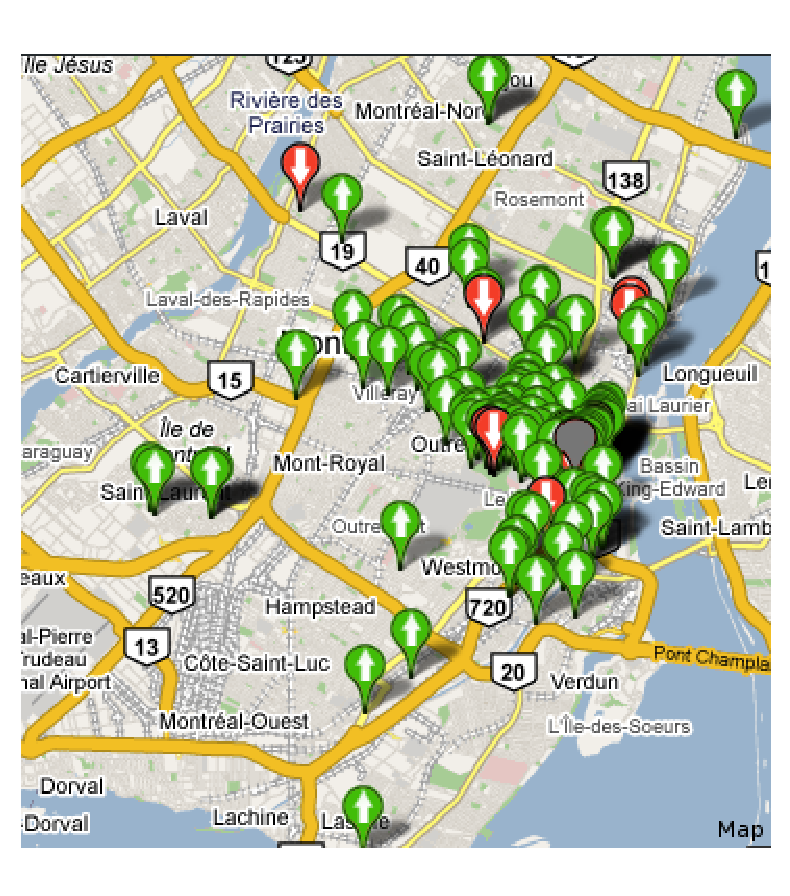
\includegraphics[scale=0.6]{./graficos/ilesansfil-core.eps}
\caption{Localiza��o dos pontos de acesso da rede na cidade de
  Montreal (citar a fonte)}
\label{graf:mapa}
\end{figure}


\section{Equa��es}


As equa��es s�o facilmente feitas e podem tamb�m ter n�meros que s�o utilizados para referenci�-las.



\begin{equation}
  \psi (u) = \int_{o}^{T} \left[\frac{1}{2}
  \left(\Lambda_{o}^{-1} u,u\right) + N^{\ast} (-u)\right] dt
\end{equation}



\begin{equation}
  \left(\frac{a^{2} + b^{2}}{c^{3}} \right) = 1 \quad
  \mbox{ se } c\neq 0 \mbox{ e se } a,b,c\in \cal{R} \enspace.
\end{equation}



\section{Algoritmos}


Os algoritmos devem ser feitos segundo o modelo abaixo. 
Para isso, usar o comando  \verb+\usepackage[ruled, portugues]{algorithm2e}+ no in�cio do arquivo principal.


\begin{algorithm}
\KwIn{o n�mero $n$ de v�rtices a remover, grafo original $G(V, E)$}
\KwOut{grafo reduzido $G'(V,E)$}
\SetLine
 $removidos \leftarrow 0$ \\
 \While {removidos $<$ n } {
   $v \leftarrow$ Random$(1, ..., k) \in V$ \\
     \For {$u \in adjacentes(v)$} {
	remove aresta (u, v)\\
	$removidos \leftarrow removidos + 1$\\
     }
     \If {h�  componentes desconectados} {
	remove os componentes desconectados\\
     }
   }
\caption{Algoritmo para remo��o aleat�ria de v�rtices}
\end{algorithm}

 % Resultados
\chapter{Conclus�es e Trabalhos Futuros} 
\label{cap:conclusoes-trabalhos-futuros}


O �ltimo cap�tulo do trabalho deve apresentar as conclus�es e apontar as possibilidade de continua��o do trabalho, ou seja, como aprimorar os resultados ou
expandir a pesquisa para novas frentes.



\section{Conclus�es} 
\label{sec:conclusoes}

\section{Trabalhos Futuros} 
\label{sec:trabalhos-futuros}


 % Conclusoes e Trabalhos Futuros
\include{apendice} % Apendices


% add the bibliography section to the table of contents
\addcontentsline{toc}{chapter}{\bibname} 
\bibliography{modelo}

\end{document}


% 
% \documentclass[protugues, brazil, a4paper,12pt]{article}
% \bibliographystyle{plain}
% \usepackage[brazil]{babel}
% \usepackage{graphicx}
% \usepackage{geometry}
% \usepackage[latin1]{inputenc}
% \usepackage[T1]{fontenc}
% \usepackage{url}
% \geometry{a4paper,left=3cm,right=3cm,top=2.5cm,bottom=2.93cm}
% \begin{document}
% \begin{titlepage}
% 
%   \vfill
% 
%   \begin{center}
%     \begin{large}
%       Universidade Federal de Minas Gerais
%     \end{large}
%   \end{center}
% 
%   \begin{center}
%     \begin{large}
%       Instituto de Ci�ncias Exatas
%     \end{large}
%   \end{center}
% 
%   \begin{center}
%     \begin{large}
%       Departamento de Ci�ncia da Computa��o
%     \end{large}
%   \end{center}
% 
%   \vfill
% 
%   \begin{center}
%     \begin{Large}
%       \textbf{PROJETO E AN\'ALISE DE ALGORITMOS \\[0.4cm] 
%         Primeiro Trabalho: dispon\'{\i}vel em:
%         \url{http://www.dcc.ufmg.br/~fbotelho/paatp3}}
% %         {http://www.dcc.ufmg.br/~fbotelho/paatp3}}               
%     \end{Large}
%   \end{center}
% 
% 
%   \vfill
% 
%   \begin{center}
%     \begin{large}
%       Fabiano Cupertino Botelho
%     \end{large}
%   \end{center}
% 
%   \begin{center}
%     \begin{large}
%       Professor - Nivio Ziviani
%     \end{large}
%   \end{center}
% 
%   \vfill
% 
%   \begin{center}
%     \begin{large}
%       Belo Horizonte \\
%       \today \\
%     \end{large}
%   \end{center}
% 
% \clearpage
% \tableofcontents 
% \end{titlepage}
% 
% 
% \section{Introdu��o}
% \cite{mar00} \\
% \cite{rp99}
% 
% \section{Algoritmo e estruturas de dados}
% 
% \section{An�lise de complexidade dos algoritmos}
% 
% \section{Apresenta��o e discuss�o dos resultados emp�ricos}
% 
% \bibliography{modelo}
% 
% \end{document}
